\documentclass[11pt]{article}

\usepackage[margin=1in]{geometry}
\usepackage{fontspec}
\setmainfont{Times New Roman}
\usepackage{graphicx}
\usepackage{booktabs}
\usepackage{array}
\usepackage{xcolor}
\usepackage{hyperref}
\usepackage{caption}
\usepackage{float}
\usepackage{amsmath}
\usepackage{enumitem}
\usepackage{titlesec}
\usepackage{fancyhdr}
\usepackage{longtable}
\usepackage{multirow}
\usepackage{parskip}

\hypersetup{colorlinks=true, linkcolor=black, citecolor=black, urlcolor=blue, pdftitle={Assignment 03 - From Data Representation to Deep Learning}}

\pagestyle{fancy}
\fancyhf{}
\fancyfoot[C]{\thepage}
\renewcommand{\headrulewidth}{0pt}
\renewcommand{\footrulewidth}{0pt}

\titleformat{\section}{\normalfont\Large\bfseries}{\thesection}{1em}{}
\titleformat{\subsection}{\normalfont\large\bfseries}{\thesubsection}{1em}{}
\titleformat{\subsubsection}{\normalfont\normalsize\bfseries}{\thesubsubsection}{1em}{}

\newcommand{\model}[1]{\textbf{#1}}
\newcommand{\code}[1]{\texttt{#1}}

\begin{document}

% ---------------------------------------------------------------------
% Cover page
% ---------------------------------------------------------------------
\begin{titlepage}
\centering
\vspace*{2cm}
{\Large INTELLIGENT SYSTEM DEVELOPMENT}\\[0.3cm]
{\Large ASSIGNMENT 03}\\[0.5cm]
{\huge \bfseries From Data Representation to Deep Learning}\\[2cm]

\begin{tabular}{ll}
Student name: & Nguyen Van Truong \\[0.5cm]
Student ID: & B23DCCE095 \\[0.5cm]
Class: & E23CNPM02 \\[0.5cm]
Team: & \underline{\hspace{7cm}} \\[0.5cm]
Lecturer: & Dinh Que Tran, Ph.D., Assoc. Prof. \\[0.5cm]
Semester: & I.2026 \\
\end{tabular}

\vfill
{\large Three intelligent systems, each trained and compared across three classical
machine learning models and one deep learning model built from scratch with NumPy.}
\end{titlepage}

\tableofcontents
\newpage

% ---------------------------------------------------------------------
\section{Executive Summary}
% ---------------------------------------------------------------------

This report builds further on the three intelligent systems developed in Assignment 02,
namely diabetes risk screening, house price prediction, and e-commerce review
classification, by adding a deep learning model built entirely from scratch in NumPy,
without any reliance on TensorFlow, PyTorch, or Keras. For each application, four models
are trained and compared on the same train/test split: three classical scikit-learn
models alongside one from-scratch feedforward network in which forward propagation, the
loss function, backpropagation, and the gradient descent update are all hand-derived and
hand-coded.

Table \ref{tab:exec-summary} lays out the three applications together with whichever of
the four trained models came out on top for that task's primary metric.

\begin{table}[H]
\centering
\caption{Executive summary across the three applications}
\label{tab:exec-summary}
\begin{tabular}{llll}
\toprule
Application & Task & Dataset & Winning model \\
\midrule
Diabetes & Binary classification & BRFSS 2019+2020, 815,711 rows & From-scratch DL \\
House price & Regression & USA real estate (600K sample) & Random Forest \\
Customer behaviour & Binary classification & Flipkart reviews, 363,261 rows & Linear SVM \\
\bottomrule
\end{tabular}
\end{table}

Two findings are worth flagging before the detailed sections below. First, the
from-scratch deep learning model actually came out ahead on the diabetes task, narrowly
beating three classical models that had each been carefully rebalanced for class
imbalance, showing that the from-scratch implementation is competitive rather than
merely functional. Second, the from-scratch network finished a clear third and fourth on
the house price and customer behaviour tasks respectively, for reasons unpacked in each
application's own section and revisited in the discussion: a heavy-tailed regression
target paired with an unbounded output layer, and a deliberately capped input vocabulary
needed to keep a dense NumPy training loop tractable. Both are genuine, explainable
limitations of a from-scratch approach rather than implementation bugs, and both are
discussed openly rather than glossed over.

% ---------------------------------------------------------------------
\section{Connection to Lecture 03: Representation Learning and Deep Learning}
\label{sec:lecture}
% ---------------------------------------------------------------------

This section is written a single time, at the framework level, so that the three
per-application sections that follow do not each need to re-derive the same mathematics.
Every from-scratch deep learning subsection below applies the ideas laid out here with its
own concrete widths and numbers, referring back to this section instead of repeating it.

\subsection{The central equation}

Lecture 03 describes a deep neural network as a chain of simple functions applied one after
another to the input:
\[
\hat{y} = (f_L \circ f_{L-1} \circ \cdots \circ f_1)(x)
\]
Each $f_\ell$ represents one layer: a linear transformation followed by a nonlinear
activation. It is the stacking of $L$ such layers that makes the network ``deep''. The
lecture's own closing summary puts it compactly: \textit{Deep Learning = Function
Composition + Representation Learning + Optimization}. Function composition is captured by
the equation above; representation learning is the notion that each layer's output
$A_\ell$ forms a new, learned representation of the input, increasingly useful for the
final task than the raw features were; optimization is the process, gradient descent, that
adjusts every layer's weights so the composed function ends up producing useful
representations rather than arbitrary ones.

\subsection{Forward propagation}

A forward pass drives a batch of input rows through every layer in turn. Each layer carries
out the same two-step operation, always in the same order: multiply first, then activate.
\[
Z_\ell = A_{\ell-1} W_\ell + b_\ell, \qquad A_\ell = g_\ell(Z_\ell)
\]
Here $A_0 = X$ denotes the input itself, $W_\ell$ and $b_\ell$ are that layer's learned
weights and biases, $Z_\ell$ is the pre-activation (the raw weighted sum before any
nonlinearity is applied), and $g_\ell$ is the layer's activation function: ReLU for every
hidden layer across all three applications in this assignment, and either sigmoid (binary
classification) or no activation at all (regression) at the output layer. Every
intermediate value produced during the forward pass is stored in a cache, since the
backward pass right after it needs those exact values to compute gradients, and
recomputing them would waste work already done once.

\subsection{Why a nonlinearity is required at all}

Without an activation function separating layers, stacking weight matrices reduces
mathematically to a single linear transformation: $X W_1 W_2 W_3$ is simply $X$ multiplied
by one combined matrix, regardless of how many weight matrices are chained together, so
depth would contribute nothing. ReLU, $\mathrm{relu}(z) = \max(0, z)$, belongs to a family
of valid nonlinearities (sigmoid, tanh, Leaky ReLU, GELU among others) that must be
deterministic, differentiable almost everywhere, and numerically well-behaved. ReLU is the
one adopted throughout this assignment's hidden layers for two practical reasons: it
behaves like an on/off switch that lets different hidden units specialize in different
input patterns, which is precisely what lets many simple pieces jointly approximate a
complicated decision boundary or price surface, and its derivative is trivial, exactly 1
where the unit is active and exactly 0 where it is not, keeping the backward pass cheap and
sidestepping the vanishing-gradient problem that an older activation such as sigmoid runs
into once stacked across many layers.

\subsection{Loss}

The loss is a single number that summarizes how wrong the network's current predictions are
across the batch. This assignment applies binary cross-entropy to the two classification
tasks (diabetes, customer behaviour) and mean squared error to the regression task (house
price), matching each task's type exactly as Lecture 03 specifies. Binary cross-entropy
penalizes a confident wrong prediction far more severely than a hedged one; mean squared
error penalizes a large miss far more heavily than a small one, since the error is squared
before averaging. Across every training loop in this assignment, computing the loss is
purely a spectator step: its numeric value is recorded only for the training-curve plots
and never feeds into the backward pass, which instead draws directly on the cached
forward-pass values.

\subsection{Backpropagation via the chain rule}

Backpropagation takes the network's final error and figures out how much each individual
weight is responsible for it, working backward from the output layer to the input layer.
At the output layer, the gradient of the loss with respect to the pre-activation collapses
to a strikingly simple form for both tasks used here, sigmoid paired with binary
cross-entropy, or a linear output paired with mean squared error:
\[
dZ_L = A_L - y
\]
This single signed number per row, the prediction minus the true label, is the entire error
signal that the rest of the network must account for. From there, every earlier layer's
gradients follow the same two-question pattern, repeated once per layer as it moves
backward:
\begin{enumerate}[nosep]
  \item How much does each weight feeding into this layer deserve to be blamed for the
    final error, proportional to how active the corresponding input was and how wrong the
    layer's own output was: $dW_\ell = A_{\ell-1}^{\top} dZ_\ell / m$, where $m$ is the
    batch size.
  \item How much of that blame should propagate to the layer before this one, and only
    through units that were actually switched on during the forward pass:
    $dA_{\ell-1} = dZ_\ell W_\ell^{\top}$, then $dZ_{\ell-1} = dA_{\ell-1} \odot
    g_{\ell-1}'(Z_{\ell-1})$.
\end{enumerate}
For a ReLU hidden layer, $g'(Z)$ equals 1 wherever $Z$ was positive during the forward pass
and 0 wherever it was not, enforcing exactly the rule that a unit which never fired cannot
be blamed for the mistake, no matter how much gradient tries to reach it. None of this
relies on an automatic differentiation library; every one of these formulas is a derivative
worked out by hand from the forward pass, which is the whole point of building the network
from scratch instead of importing one.

\subsection{Gradient descent and weight initialization}

Once every gradient is known, the update step amounts to plain gradient descent, applied to
every weight and bias in the network:
\[
W_\ell \leftarrow W_\ell - \eta \, dW_\ell, \qquad b_\ell \leftarrow b_\ell - \eta \, db_\ell
\]
where $\eta$ is the learning rate. Training follows this four-step cycle, forward, loss (a
spectator step), backward, update, repeated over many epochs; each repetition only nudges
the weights a small step in a locally better direction, which is why so many repetitions
are needed before the loss visibly flattens out.

Before any of this can run, the weights need a starting point. Setting every weight to zero
would make every neuron in a layer compute an identical output and receive an identical
gradient forever, so the starting values must be random. Plain unscaled randomness
introduces a second problem once layers are stacked: a layer that happens to shrink
whatever passes through it fades the signal toward zero by the third layer, while one that
happens to amplify it blows the signal up, purely as a side effect of how the initial
weights were drawn. He initialization, applied throughout this assignment per the
lecture's own specification, addresses this by scaling the random starting weights so a
layer's output keeps roughly the same variance as its input:
\[
W_\ell \sim \mathcal{N}(0, 1) \times \sqrt{\dfrac{2}{\mathrm{fan\_in}_\ell}}, \qquad b_\ell = 0
\]
The factor of 2 exists specifically to compensate for ReLU: because ReLU zeroes out every
negative value, it wipes out roughly half of the variance reaching it on average, so the
initial weights are scaled up to make up for that. An older scheme meant for smoother
activations such as sigmoid or tanh, Xavier/Glorot initialization, uses
$1/\mathrm{fan\_in}$ instead, without that factor of 2. Biases start at exactly zero,
which is safe since it is the random weights, not the biases, that break the symmetry
between neurons in a layer.

\subsection{What ``from scratch'' means in this assignment}

All three applications below satisfy the same constraint: no \code{tensorflow},
\code{torch}, or \code{keras} import appears anywhere in the deep learning code, and
forward propagation, the loss function, backpropagation, and the gradient descent update
are each derived by hand and implemented directly in NumPy. scikit-learn is used only for
the three classical models in each application, never for the deep learning model itself.
\code{RANDOM\_SEED = 42} is fixed wherever splits, shuffles, or weight initialization
occur, and every scaler or vectorizer is fit on the training split alone, then applied
unchanged to the test split, so no information from the held-out test data leaks into
training.

% ---------------------------------------------------------------------
\section{Diabetes: Binary Classification}
\label{sec:diabetes}
% ---------------------------------------------------------------------

\subsection{Problem description}

This application predicts whether a BRFSS (Behavioral Risk Factor Surveillance System)
survey respondent has diabetes or pre-diabetes, based on their self-reported health and
demographic answers. It takes the binary classification shape that Lecture 03 calls
Application 1: patient data passes through a learned representation to produce
$P(\text{diabetes})$.

\subsection{Dataset}

The dataset combines two full annual files from the Kaggle dataset:
\begin{center}
\small\url{https://www.kaggle.com/datasets/spandanjit2005/brfss-diabetes-indicator-dataset}
\end{center}
\texttt{DATASET\_2019.csv} (416,661 rows) and \texttt{DATASET\_2020.csv} (399,050 rows),
concatenated into one 815,711-row table. The two years did not share an identical schema:
the 2019 file includes two columns, \verb|high_bp_00| and \verb|high_cholesterol_00|, that
are entirely absent from the 2020 file. This reflects a structural difference between the
two years' questionnaires rather than a random missing-value issue, so both columns are
dropped from the combined dataset instead of being imputed. No rows had to be dropped for a
missing or malformed target, since every one of the 815,711 rows carries a valid
three-class diagnosis, leaving the cleaned dataset at the full 815,711 rows.

The target is BRFSS's own \verb|diabetes| field, originally three classes
(non-diabetic / pre-diabetic / diabetic), collapsed to binary: 0 for non-diabetic and 1 for
pre-diabetic or diabetic combined, matching both Assignment 02's framing and the lecture's
binary decision rule ($\hat{y} \geq 0.5 \Rightarrow$ diabetes). The resulting target carries
meaningful imbalance: 84.4\% of respondents are non-diabetic while 15.6\% are diabetic or
pre-diabetic (Figure \ref{fig:diabetes-eda-target}).

\subsection{Data understanding and cleaning}

Two columns, \verb|avg_drinks_p_day_00| and \verb|poor_health_days_00|, are missing for
roughly half of all respondents. Both are conditionally asked questions within the BRFSS
questionnaire (asking about average drinks per day only makes sense for someone who already
reported drinking), so the missingness reflects survey design rather than a data quality
problem, and both columns are dropped rather than imputed. \verb|income_00| is missing for
about one in five respondents, a common pattern for income questions in surveys, and is
retained with median imputation instead of being dropped. Two BRFSS sentinel values were
also identified and cleaned: \verb|weight_00 == 999| (15 rows) and \verb|bmi_00 > 100|
(78 rows) are placeholder codes marking implausible readings rather than genuine outliers,
so they are set to missing before imputation.

Exploratory analysis confirmed several expected clinical relationships within the data.
Respondents with diabetes or pre-diabetes show a visibly higher average BMI than
non-diabetic respondents, consistent with the well-established link between excess body
weight and type 2 diabetes risk. Self-reported general health tracks diabetes status almost
monotonically: respondents rating their health ``excellent'' or ``very good'' report
diabetes at a much lower rate than those rating it ``fair'' or ``poor,'' which is also why
this ordinal field is kept as a numeric code instead of one-hot encoded, since the ordering
itself carries signal. The diabetes rate by survey year turned out close between 2019
(15.97\%) and 2020 (15.20\%), too small a gap by itself to justify keeping \verb|year| as a
feature, but it was retained regardless: since \verb|high_bp_00| and
\verb|high_cholesterol_00| had to be dropped over the schema mismatch above, \verb|year| is
one of the few remaining signals that could let a model pick up on any residual survey-wave
effect, so leaving that decision to the models themselves costs little.

\begin{figure}[H]
\centering
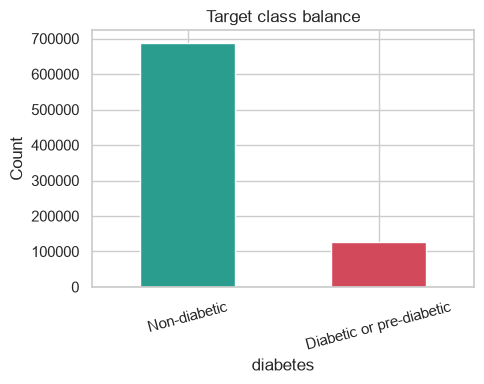
\includegraphics[width=0.5\linewidth]{images/diabetes_eda_class_balance.png}
\caption{Target class balance after collapsing the three original diabetes categories to
binary. Positives sit well under a quarter of the data, which is why accuracy alone would
be a misleading way to judge these models.}
\label{fig:diabetes-eda-target}
\end{figure}

\subsection{Representation}

Every remaining column falls into one of four buckets, following the rule that a field is
only one-hot encoded if its categories carry no natural order. Continuous measurements
(age, weight, height, BMI, days of poor physical or mental health) are median-imputed and
standardized with a scaler fit only on the training split. Ordinal survey fields already
coded as small integers (education level, income bracket, general health, time since last
checkup) are median-imputed but left unscaled, since one-hot encoding them would discard
the ordering that gives them their value. Boolean yes/no fields (exercise, smoking history,
alcohol use, personal history of stroke, heart attack, or coronary disease, cost barrier to
care) are mapped to 0/1 and imputed with the majority answer. Genuinely unordered
categorical fields (sex, race, marital status, employment status, personal doctor access)
are one-hot encoded, with missing values folded into their own ``Unknown'' category. The
\verb|year| column is kept as a 0/1 flag (2020 vs. 2019) rather than the literal survey
year integer: left as a raw value, \verb|year| would enter the feature matrix at a scale
of roughly 2020, dwarfing every standardized or small-integer feature next to it and badly
distorting the from-scratch network's forward pass, a problem discussed further in Section
\ref{sec:discussion}.

This yields a feature matrix 49 columns wide before scaling. The 80/20 train/test split
(\texttt{RANDOM\_SEED = 42}, stratified on the target) produces 652,568 training rows and
163,143 test rows, with the same 15.59\% positive rate preserved across both splits.

\subsection{Classical machine learning models}

Three classical models were fit on the same training split, each representing a different
inductive bias: \model{Logistic Regression} as a linear, cheaply interpretable baseline;
\model{Random Forest}, the model Assignment 02 deployed for this application, retained for
continuity; and \model{Gradient Boosting}, which tests whether the extra sequential-
correction capacity beyond simple bagging helps on this feature set.

Because the target is imbalanced, a plain fit at the default 0.5 decision threshold would
be trained to minimize an average loss dominated almost entirely by the majority class,
quietly settling into a model that rarely predicts ``diabetic'' at all. All three classical
models, along with the from-scratch network below, were therefore trained with balanced
sample weights computed as $n_{\text{total}} / (n_{\text{classes}} \times n_{\text{class}})$,
so that a mistake on a diabetic row costs as much in the total training objective as a
mistake on a non-diabetic row, even though diabetic rows are roughly five times rarer. This
changes the loss surface that gradient descent (or the tree models' equivalent internal
optimization) actually descends, rather than merely adjusting the decision threshold after
the fact.

\begin{table}[H]
\centering
\caption{Diabetes: classical model results (balanced sample weighting), test set}
\begin{tabular}{lrrrr}
\toprule
Model & Accuracy & Precision & Recall & F1 \\
\midrule
Logistic Regression & 0.7236 & 0.3318 & 0.7617 & 0.4622 \\
Random Forest & 0.7146 & 0.3272 & 0.7861 & 0.4621 \\
Gradient Boosting & 0.7149 & 0.3279 & 0.7893 & 0.4633 \\
\bottomrule
\end{tabular}
\end{table}

\begin{figure}[H]
\centering
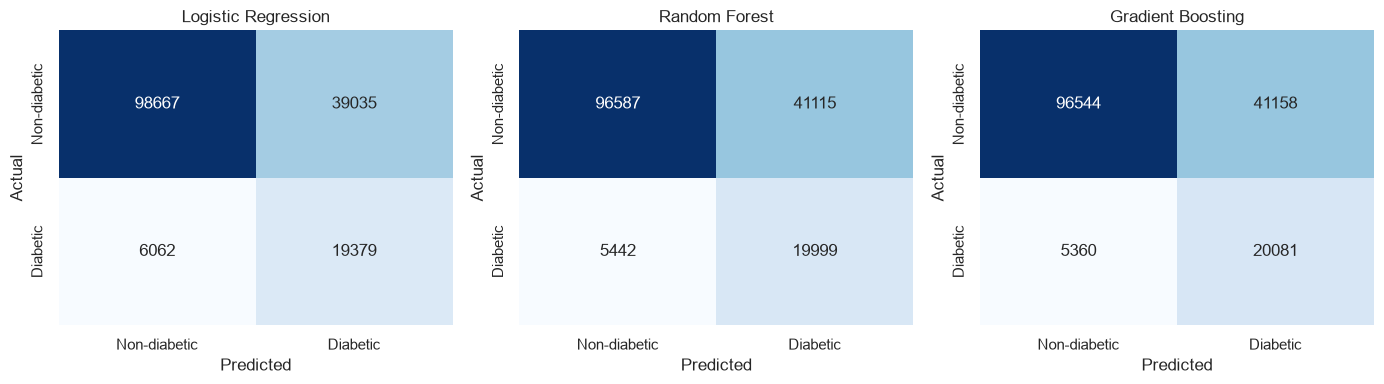
\includegraphics[width=\linewidth]{images/diabetes_classical_confmat.png}
\caption{Confusion matrices for the three classical models on the diabetes test set.}
\end{figure}

Balanced weighting lifted recall from an 8.5-17.9\% pre-weighting range to the 74-79\%
range shown above, meaning these models now catch roughly three-quarters of actual
diabetic or pre-diabetic respondents rather than a small fraction of them. That gain came
at a cost: precision fell from a 0.53-0.61 pre-weighting range down to roughly 0.33, and
accuracy dropped from around 85\% into the low 70s, a genuine trade-off discussed further
below.

\subsection{From-scratch deep learning model}

The network follows a $49 \to 49 \to 24 \to 1$ architecture, computed at runtime from
however many columns the one-hot encoding actually produces rather than hardcoded, with
ReLU activations on both hidden layers, a sigmoid output, and binary cross-entropy loss,
exactly matching the classification setup from Section \ref{sec:lecture}. The first hidden
layer is sized close to the input width and the second at roughly half of that, mirroring
the narrowing pattern of the reference tutorial's own $8 \to 16 \to 8 \to 1$ example scaled
up to this application's wider input. Because the feature matrix is fully dense and modest
in width, training relies on full-batch gradient descent: one forward pass over all
652,568 training rows, one backward pass, one weight update, per epoch, with no
mini-batching required.

The balanced sample weights used for the classical models carry over directly into the
from-scratch implementation: the binary cross-entropy loss function accepts an optional
per-row \code{weights} argument that multiplies each row's penalty before averaging, and
the backward pass multiplies the output-layer error signal $dZ_3 = (A_3 - y)$ by that same
weight array, so the imbalance correction propagates through every downstream gradient
exactly as it does for the classical models.

The learning rate and epoch count were settled through direct benchmarking rather than
guesswork: a larger candidate rate caused the loss to spike on the very first update
(pre-activations too large for sigmoid to handle cleanly) before settling into a noticeably
worse minimum, while smaller rates converged more slowly without ever reaching a better
one. \texttt{LEARNING\_RATE = 0.1} and \texttt{EPOCHS = 300} turned out to be the values
that let the loss curve fall furthest within a reasonable runtime for a plain NumPy loop
over 650,000+ rows.

\begin{figure}[H]
\centering
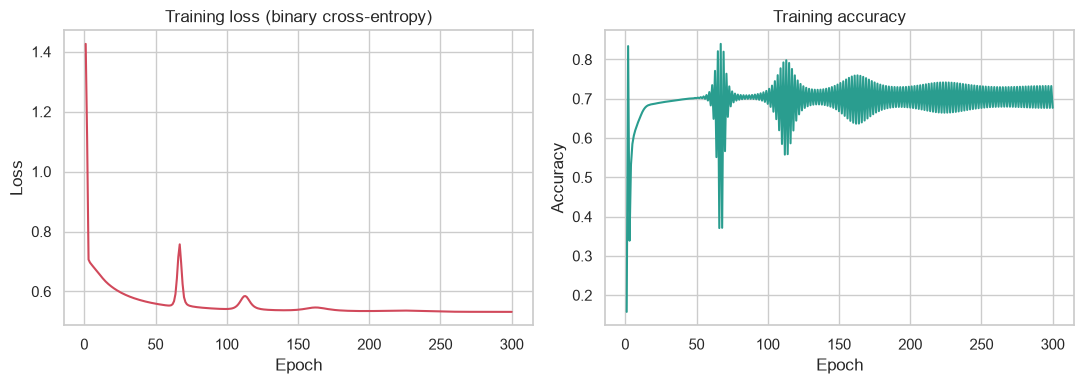
\includegraphics[width=\linewidth]{images/diabetes_dl_loss_acc.png}
\caption{Training loss (binary cross-entropy) and training accuracy per epoch for the
from-scratch diabetes network. Both curves flatten out well before epoch 300, indicating
the network converged rather than being cut off mid-training.}
\end{figure}

\begin{table}[H]
\centering
\caption{Diabetes: from-scratch DL model results, test set}
\begin{tabular}{lrrrr}
\toprule
Model & Accuracy & Precision & Recall & F1 \\
\midrule
From-scratch DL & 0.7343 & 0.3388 & 0.7401 & 0.4648 \\
\bottomrule
\end{tabular}
\end{table}

\subsection{4-model comparison}

\begin{figure}[H]
\centering
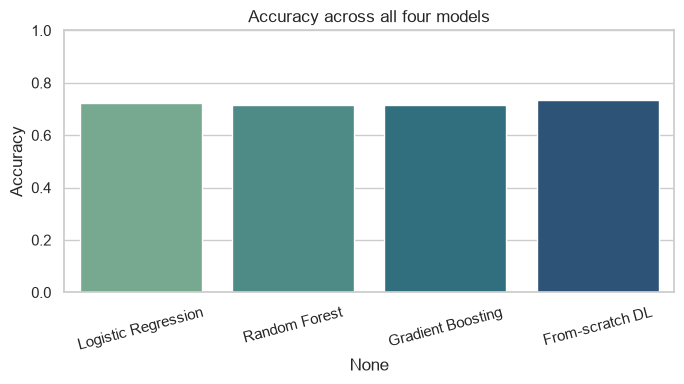
\includegraphics[width=0.7\linewidth]{images/diabetes_compare_accuracy.png}
\caption{Accuracy across all four diabetes models.}
\end{figure}

\begin{figure}[H]
\centering
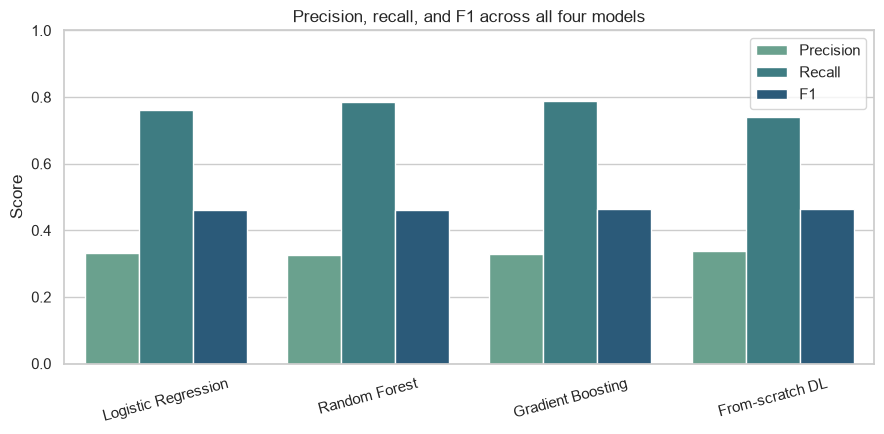
\includegraphics[width=\linewidth]{images/diabetes_compare_prf1.png}
\caption{Precision, recall, and F1 across all four diabetes models.}
\end{figure}

The from-scratch network finishes on top by F1 at 0.4648, just ahead of Gradient Boosting
(0.4633), Logistic Regression (0.4622), and Random Forest (0.4621). What stands out more
than the ranking itself is how tightly bunched all four numbers are, within half a
percentage point of one another, a dramatic shift from the pre-weighting comparison where
the same four models spread from 0.1494 to 0.2712. That collapse in spread follows directly
from balanced weighting: every model is now pushed toward the same class trade-off by
construction, so most of what previously separated these four models was really a
difference in how aggressively each one's default training happened to favor the majority
class, not a difference in how well each could actually distinguish the two classes.
Within that shared trade-off, the from-scratch network's small edge is a reasonable
outcome: its two ReLU hidden layers grant it more representational flexibility than
Logistic Regression's single linear boundary, without the tree ensembles' tendency to carve
the feature space into many small, axis-aligned regions that can each overfit their own
local slice of training data.

The precision cost deserves a concrete look. For the from-scratch network, the confusion
matrix works out to roughly 36,700 false positives against about 18,800 true positives,
meaning nearly two people are flagged as at-risk for every one who actually has diabetes or
pre-diabetes. Since this model relies on self-reported survey answers rather than a
diagnostic test, a false positive here only costs one unnecessary follow-up screening test
(typically fasting glucose or HbA1c, routine and inexpensive), whereas a false negative
risks years of undetected disease progression toward complications that are far more
expensive and less reversible. That asymmetry is why real screening tools are deliberately
tuned to catch more true cases even at the cost of more false alarms, which is the
reasoning behind keeping balanced weighting as the final choice for every model in this
comparison, not because higher recall is automatically better in general, but because it
suits this problem's specific cost structure.

\newpage
% ---------------------------------------------------------------------
\section{House Price: Regression}
\label{sec:house_price}
% ---------------------------------------------------------------------

\subsection{Problem description}

This application predicts a real-estate listing's price in US dollars from its attributes:
bedroom and bathroom counts, lot size, house size, location, and sale history. It takes the
regression shape Lecture 03 calls Application 2: house attributes pass through a learned
representation to produce a price.

\subsection{Dataset}

The dataset is \texttt{realtor-data-sample.csv}, a 600,000-row seeded sample
(\texttt{RANDOM\_SEED = 42}) of the 2,226,382-row source dataset:
\begin{center}
\small\url{https://www.kaggle.com/datasets/ahmedshahriarsakib/usa-real-estate-dataset}
\end{center}
republished as:
\begin{center}
\small\url{https://www.kaggle.com/datasets/minorin2847/usa-real-estate-600k-sample}
\end{center}
so re-runs do not need to re-sample, and the data genuinely reflects US-market listings.
After dropping 488 rows with a missing or non-positive price, the cleaned dataset used for
splitting and training comes to 599,512 rows.

\subsection{Data understanding and cleaning}

The raw price distribution is heavily right-skewed: most homes cluster within a normal
price range, but a long tail of multi-million-dollar properties stretches the axis so far
that the bulk of the data gets squeezed into a sliver on the left (Figure
\ref{fig:hp-eda-price}). Taking $\log(1+\text{price})$ turns that into something close to a
bell curve, and training on the log-transformed target rather than raw dollars keeps the
loss from being dominated by getting a handful of very expensive homes exactly right at the
expense of everything else: without the log transform, a squared-error loss would treat a
\$50,000 miss on a \$300,000 home as almost negligible next to a \$50,000 miss on a
\$5,000,000 home, even though the first miss is arguably the more serious one in relative
terms.

\begin{figure}[H]
\centering
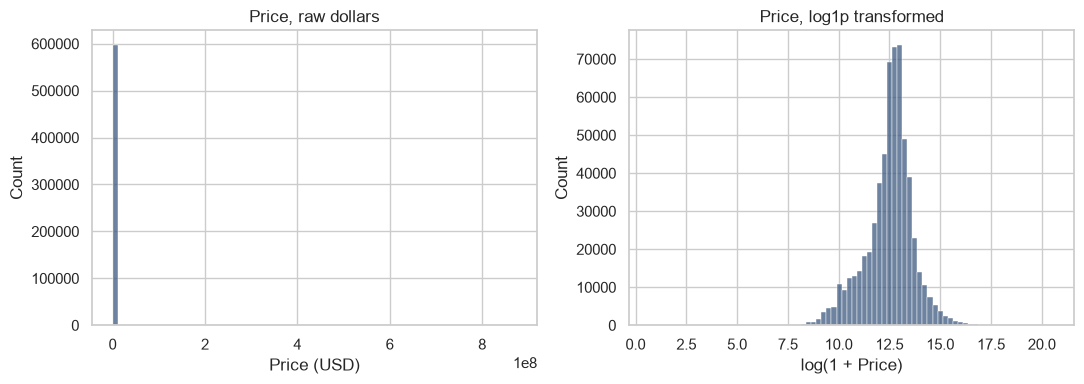
\includegraphics[width=\linewidth]{images/house_price_eda_price_dist.png}
\caption{Price distribution, raw dollars versus $\log(1+\text{price})$. The log transform
turns the heavy right tail into an approximately bell-shaped distribution, which is why the
target is trained in log space and converted back to dollars with \code{expm1} for every
reported metric.}
\label{fig:hp-eda-price}
\end{figure}

House size correlates with price more strongly (0.487) than bedroom or bathroom count do on
their own, which makes sense since size is a direct physical measurement while bedroom and
bathroom counts are coarser proxies for it. Median price also varies enormously by state,
several times higher in the most expensive markets than in the cheapest, which argues for
keeping \verb|state| in the feature set rather than treating location as noise. A handful
of physically implausible values were identified and treated as missing rather than
dropped outright, to avoid losing otherwise-valid price and location data: bedrooms above
20 (149 rows), bathrooms above 20 (77 rows), lot size above 1,000 acres (431 rows), and
house size above 50,000 square feet (33 rows). \verb|acre_lot| and \verb|house_size| both
turned out to be far more heavily tailed than a plain standard scaler can handle (the
lot-size standard deviation is roughly 27, nearly a hundred times the 0.32-acre median), so
both columns received the same \verb|log1p| treatment already applied to price before
standardization.

\verb|prev_sold_date| is missing for 41.4\% of listings, which at first glance looks like a
data quality problem, but the pattern is fully explained by listing status: every
\verb|ready_to_build| listing is missing it (the property has not been built yet, so it
cannot have a previous sale), while every \verb|sold| listing has one. Rather than drop the
column, it was engineered into two features: a binary \verb|had_prev_sale| flag and a
numeric \verb|days_since_prev_sale| for rows where a previous sale exists, so the flag
carries the ``never sold'' signal instead of a suspicious zero or an arbitrary placeholder.

\subsection{Representation}

\verb|brokered_by| and \verb|street| were dropped outright, since both are anonymized
numeric IDs in the source data carrying no generalizable signal. \verb|status| and
\verb|state| are both genuinely unordered categories with a manageable number of values
(3 and 55 respectively), so both are one-hot encoded, producing 58 one-hot columns.
\verb|city| tells a different story, with close to 15,000 distinct values (14,268 seen in
the training split); one-hot encoding it would add thousands of mostly-empty columns, so
each city is instead replaced with how often it appears in the training data, a frequency
encoding that preserves location signal without exploding the feature count (782 test-set
cities unseen in training are encoded as 0). \verb|zip_code| carries even higher
cardinality and captures much of the same location information once state and city
frequency are already present, so it is dropped rather than frequency-encoded as well,
avoiding two highly correlated location encodings competing for the same signal. The city
frequency count itself is log-transformed (the same heavy-tailed shape issue as lot size
and house size) before joining the other continuous columns in a single
\verb|StandardScaler| fit on the training split.

The final feature matrix spans 65 columns: 6 standardized continuous features (bedrooms,
bathrooms, log lot size, log house size, days since previous sale, log city frequency), the
binary \verb|had_prev_sale| flag, and 58 one-hot status/state columns. The 80/20 split
yields 479,609 training rows and 119,903 test rows.

\subsection{Classical machine learning models}

\model{Linear Regression} serves as the simplest possible baseline, assuming log-price is a
straight-line combination of every feature with no interactions. \model{Random Forest}, the
model Assignment 02 deployed for this application, is retained for continuity, with
\texttt{max\_depth=14} giving its 200 trees room to split on fine-grained location and size
combinations. \model{Gradient Boosting} grows 150 shallow trees (\texttt{max\_depth=3})
sequentially, each one correcting the residual error left by the trees before it, moderated
by a \texttt{learning\_rate=0.1} so the corrections accumulate smoothly.

\begin{table}[H]
\centering
\caption{House price: classical model results (dollars), test set}
\begin{tabular}{lrrr}
\toprule
Model & RMSE & MAE & $R^2$ \\
\midrule
Linear Regression & 9,092,233 & 397,323 & $-48.3632$ \\
Random Forest & 1,004,048 & 225,937 & 0.3980 \\
Gradient Boosting & 1,128,427 & 251,391 & 0.2397 \\
\bottomrule
\end{tabular}
\end{table}

\begin{figure}[H]
\centering
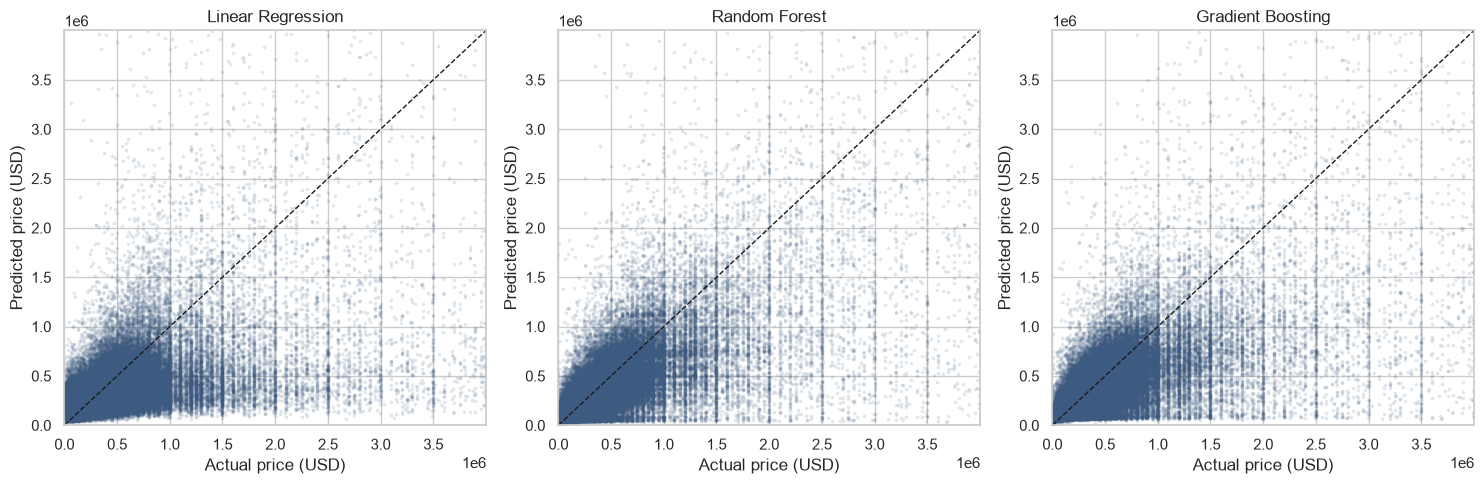
\includegraphics[width=\linewidth]{images/house_price_classical_scatter.png}
\caption{Predicted versus actual price for the three classical models (99th-percentile
axis limit for readability). All three track the diagonal well at lower prices and spread
further away as price climbs into the sparser, more idiosyncratic high end.}
\end{figure}

\subsection{From-scratch deep learning model}

The network follows a $65 \to 64 \to 32 \to 1$ architecture, with ReLU activations on both
hidden layers. Since this is regression rather than classification, the output layer omits
the sigmoid, house prices are not probabilities, so the final layer is left as a plain
linear combination ($A_3 = Z_3$), and the loss is mean squared error rather than binary
cross-entropy. The hidden layers are wider relative to the input than the diabetes
network's, since the relationship between listing attributes and price is plausibly more
nonlinear (location and size interact in ways a simple weighted sum cannot capture well),
so the extra capacity gives the network room to represent those interactions. The gradient
of mean squared error with respect to the linear output reduces to the same simple form as
in the classification case, $dZ_3 = A_3 - y$ (up to a constant absorbed into the learning
rate), so the backward pass is structurally identical to the diabetes network's, just
derived from a different loss.

Reaching a stable training run took genuine trial and error, and the failure mode along the
way is worth naming since it differs from the scale problem the representation section
above already fixed. At a learning rate of 0.3, the first few updates pushed every neuron
in the second hidden layer into permanently outputting zero for every training row, a
``dead ReLU'' collapse: once a unit's pre-activation turns negative for every row, its
gradient becomes zero everywhere too, so gradient descent has no way to revive it, and the
network gets stuck predicting a constant close to the mean log-price for the rest of
training. Lowering the learning rate to \texttt{LEARNING\_RATE = 0.01} avoided the
collapse entirely (verified directly: zero dead units in the second layer, checked
throughout training) and let the loss keep decreasing across \texttt{EPOCHS = 2000}
full-batch updates.

\begin{figure}[H]
\centering
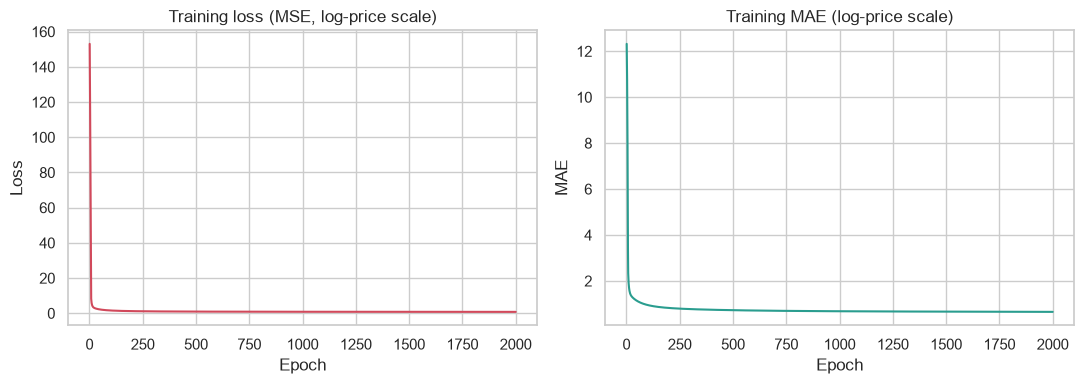
\includegraphics[width=\linewidth]{images/house_price_dl_loss_mae.png}
\caption{Training loss (MSE, log-price scale) and training MAE (log-price scale) per epoch
for the from-scratch house price network.}
\end{figure}

\begin{table}[H]
\centering
\caption{House price: from-scratch DL model results (dollars), test set}
\begin{tabular}{lrrr}
\toprule
Model & RMSE & MAE & $R^2$ \\
\midrule
From-scratch DL & 1,877,302 & 293,579 & $-1.1044$ \\
\bottomrule
\end{tabular}
\end{table}

\subsection{4-model comparison}

\begin{figure}[H]
\centering
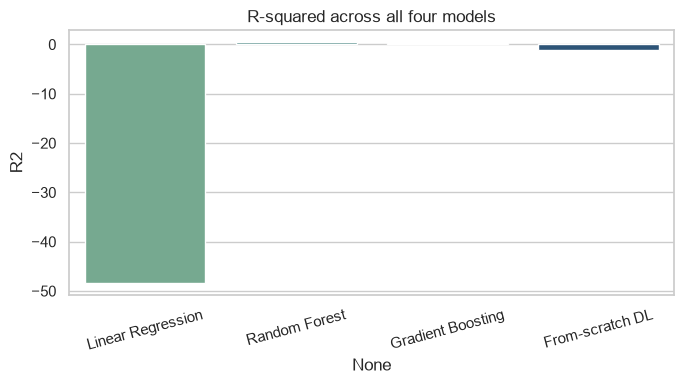
\includegraphics[width=0.7\linewidth]{images/house_price_compare_r2.png}
\caption{$R^2$ across all four house price models.}
\end{figure}

\begin{figure}[H]
\centering
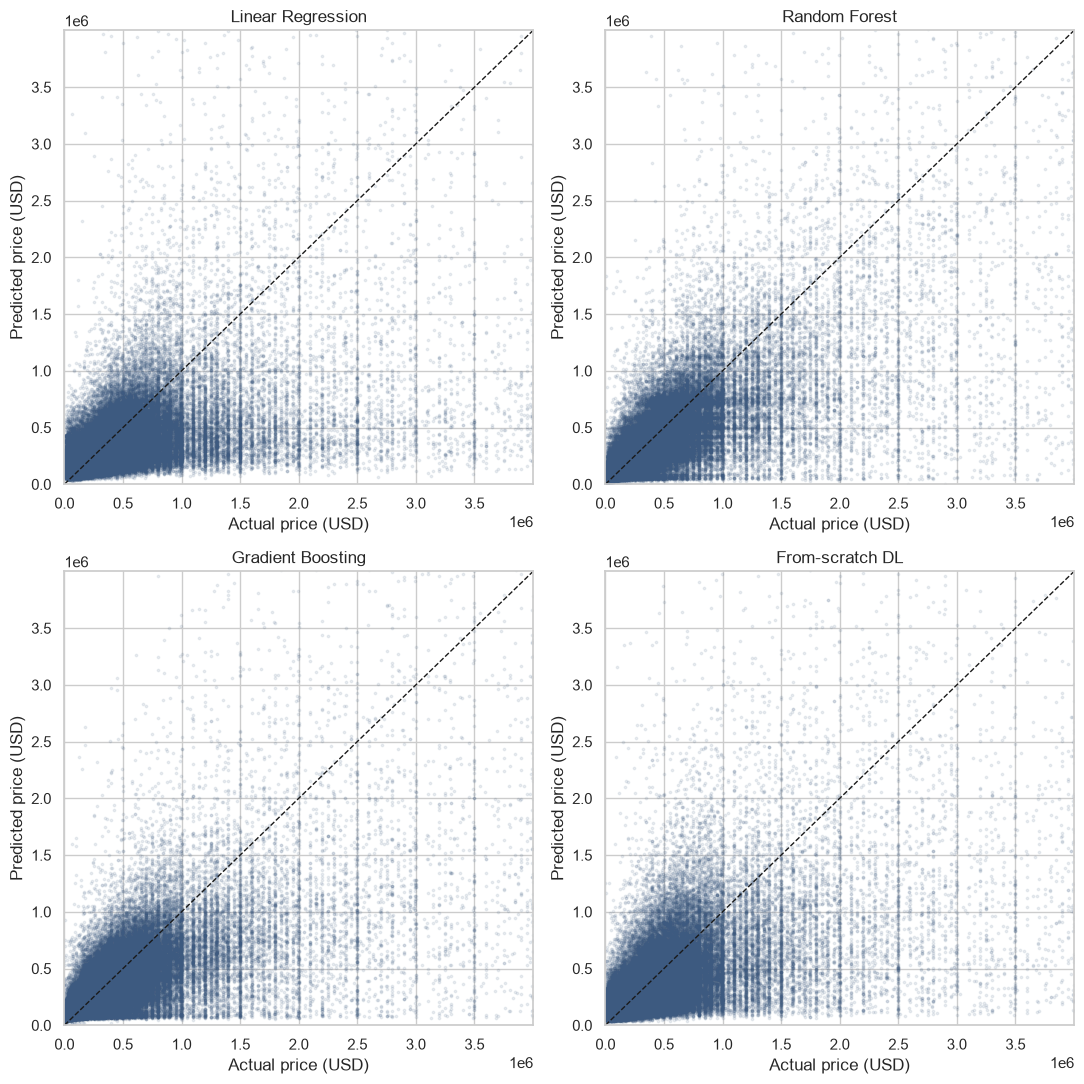
\includegraphics[width=\linewidth]{images/house_price_compare_scatter_grid.png}
\caption{Predicted versus actual price, all four models, shared dollar axis.}
\end{figure}

Random Forest wins on every metric (RMSE 1,004,048; MAE 225,937; $R^2$ 0.3980), ahead of
Gradient Boosting ($R^2$ 0.2397). The from-scratch network places third ($R^2 = -1.1044$),
with Linear Regression finishing last by a wide margin ($R^2 = -48.3632$). That last figure
is the one worth pausing on: judged by MAE alone, Linear Regression does not look
catastrophic; it is only $R^2$ that reveals just how badly it is actually performing.

The reason traces back to how heavy-tailed price itself is: the training data has a median
of roughly \$315,000, a 99th percentile around \$4.2 million, and a maximum of \$875
million. Training on log-price tames that skew for fitting purposes but does not remove
the tail, it merely relocates where the tail causes damage. Every prediction is passed back
through \code{expm1} to convert a log-price into dollars, and \code{expm1} is a convex,
explosive function: a modest error in log-space, applied to a listing whose true price is
already in the tens of millions, balloons into an enormous error in dollar-space, and
$R^2$, built from squared error, ends up dominated by whichever handful of rows carry the
largest dollar-space misses.

What separates the two tree ensembles from Linear Regression and the from-scratch network
is less about smaller log-space error and more about a structural limit on how wrong a
single prediction can get. A tree's prediction for any row is an average of training
log-prices from whichever leaf that row lands in, so it can never output a value far
outside the range its training leaves actually contained. Linear Regression has no such
ceiling, its output is an unbounded linear combination of the input features, and the
from-scratch network's output layer shares exactly the same structure, a plain linear
combination with no squashing activation, since nothing here calls for one the way sigmoid
was needed for the classification tasks. That the network still beats Linear Regression by
a wide margin on all three metrics, despite sharing this structural weakness, suggests the
two ReLU hidden layers are doing real work, fitting the bulk of the log-price distribution
with a piecewise-nonlinear function rather than a single flat plane, even though neither
model gets the tree ensembles' built-in protection against an occasional wild
extrapolation.

\newpage
% ---------------------------------------------------------------------
\section{Customer Behaviour: Binary Classification}
\label{sec:customer_behaviour}
% ---------------------------------------------------------------------

\subsection{Problem description}

This application predicts whether a Flipkart product review reflects a recommendation,
defined as a rating of 4 or 5 stars, based on the review's text and the product's price. It
takes the binary classification shape Lecture 03 calls Application 3: text passes through
a learned representation to produce a sentiment or recommendation signal.

\subsection{Dataset}

The dataset is \texttt{flipkart\_reviews.csv} from the Kaggle dataset:
\begin{center}
\small\url{https://www.kaggle.com/datasets/niraliivaghani/flipkart-dataset}
\end{center}
loaded as 363,261 rows across 5 columns
(\texttt{Product\_name}, \texttt{Price}, \texttt{Rate}, \texttt{Review},
\texttt{Summary}). Flipkart was deliberately chosen as a different e-commerce platform
(general merchandise spanning 75+ categories) rather than reusing the Sephora review data
from Assignment 02, so as to work with a genuinely different review vocabulary and product
mix. After dropping rows with an unparseable rating, a missing \texttt{Summary}, or a
missing price, the cleaned dataset comes to 361,233 rows (2,028 dropped, 0.56\%).

\subsection{Data understanding and cleaning}

The \texttt{Price} column arrived corrupted: the source file's Rupee symbol did not survive
export and left behind stray bytes that broke direct numeric conversion for every single
row (363,261 out of 363,261 rows failed to parse as a plain number before cleaning). A
regex that strips everything except digits and the decimal point recovers a normal-looking
retail price distribution once applied. \texttt{Rate} also loads as text rather than a
clean integer, with 44 rows carrying an unparseable or out-of-range value, which are
dropped during cleaning.

Ratings pile up heavily at 5 stars (Figure \ref{fig:cb-eda-target}), and the derived
\texttt{is\_recommended} target inherits that skew: 76.6\% of reviews are labeled
recommended. Reviews with a low rating also tend to run noticeably longer than five-star
reviews, which fits how people actually write reviews: a happy customer often just says
``nice product,'' while a disappointed one tends to spell out exactly what went wrong.

\begin{figure}[H]
\centering
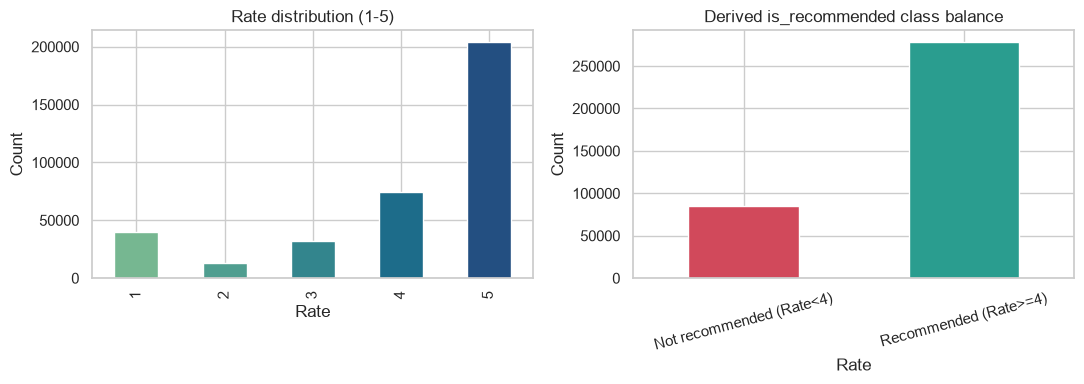
\includegraphics[width=\linewidth]{images/cb_eda_class_balance.png}
\caption{Rate distribution (1-5) and the derived \texttt{is\_recommended} class balance.}
\label{fig:cb-eda-target}
\end{figure}

The most consequential finding in this application's EDA concerned which text field the
representation should be built from. \texttt{Review} looks like ordinary free text at a
glance, but overwhelmingly consists of a small set of one- or two-word stock phrases
repeated tens of thousands of times each (``Wonderful'' appears 18,567 times, ``Awesome''
11,501 times, ``Great product'' 11,300 times), with only 3,842 unique review texts across
363,261 rows, 1.06\%. \texttt{Summary}, by contrast, is present in nearly every row
(99.44\%) and far richer, with 165,850 unique texts among the rows that have one, 45.9\%
(Figure \ref{fig:cb-eda-repetition}).

\begin{figure}[H]
\centering
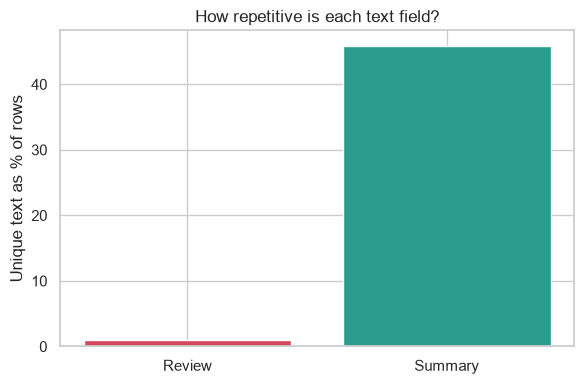
\includegraphics[width=0.6\linewidth]{images/cb_eda_text_repetitiveness.png}
\caption{Unique text as a percentage of rows, Review versus Summary. Review is overwhelmingly
repeated boilerplate; Summary is far richer.}
\label{fig:cb-eda-repetition}
\end{figure}

This gap matters for more than variety's sake. A model trained and evaluated on such a
repetitive text field is not really being tested on new language during evaluation, since
most of what shows up in the test split is a word-for-word copy of something already seen
in training, so the evaluation ends up measuring memorization of a small boilerplate
vocabulary rather than genuine generalization. An earlier version of this notebook that used
\texttt{Review} directly as the TF-IDF input scored close to 0.99 F1 across all four
models, a result investigated directly once it looked suspiciously high: 99.1\% of
test-set \texttt{Review} texts turned out to appear verbatim in the training set. Switching
the representation to \texttt{Summary} drops that train/test exact-text overlap to 59.7\%,
still non-trivial (short one-word summaries like ``Good'' or ``Nice'' still repeat a lot),
but a real improvement rather than a cosmetic one, and this is the representation actually
used in the results reported below.

A second, separate factor also keeps these scores high even after the Summary switch. For
roughly three in four rows, the exact Summary text is at least 95\% associated with a
single label across every other row sharing that same text (``Excellent'' is recommended
98.7\% of the time it appears, ``Very good'' 96.2\%, even a plain ``Good'' 88.2\% of the
time despite being the single most common Summary in the dataset). This is not evaluation
leakage the way the Review-text overlap was, since it does not depend on the model having
seen that literal string during training; it is a genuine property of how people write
these summaries: someone who types ``Excellent'' is overwhelmingly likely to have also
given 4 or 5 stars. The exception is informative too: ``Ok'' sits at only 62.5\% purity,
close to a coin flip, exactly what a genuinely ambiguous word should look like, which is
reassuring evidence that the purity pattern reflects real sentiment-language correlation
rather than a methodology problem.

A full-row duplicate check also turned up a large number of exact duplicate rows
(identical product, price, rating, and text). These were kept rather than dropped: short
generic reviews really do get written repeatedly by different real buyers of the same
popular item, so collapsing them would throw away genuine signal about how common that
kind of review is, not merely clean up parsing artifacts.

\subsection{Representation}

\texttt{Summary} text becomes a TF-IDF vector over unigrams and bigrams, chosen over
\texttt{Review} for the leakage and vocabulary-richness reasons established above. Two
separate vectorizers are fit, since the two model families need different vocabulary
sizes: the classical models get the full vocabulary with no artificial cap, 416,770 unique
terms, since scikit-learn's sparse linear models handle that size comfortably given the
matrix stays sparse all the way through training. The deep learning model instead gets a
vocabulary capped at 5,000 terms, roughly 1.2\% of the full vocabulary, because a dense
NumPy forward and backward pass has no sparse representation to lean on: every column
becomes a real, materialized number for every row, so all 416,770 of them would be far too
slow and memory-hungry to train from scratch. This cap is a deliberate, stated trade-off,
and it is also the most direct explanation for why the from-scratch model trails the
classical ones in the comparison below: it only reads a small fraction of the vocabulary
the linear models get to see. \texttt{Price}, once cleaned into a number, is standardized
with a scaler fit only on the training split. \texttt{Product\_name} is left out of the
feature set entirely, being high-cardinality free text (a small set of popular items
dominate review volume, with most other products appearing only a handful of times each)
that would mostly encourage memorization rather than generalization. \texttt{Review}
itself is dropped rather than combined with \texttt{Summary}, for the same leakage reason:
adding it back would reopen the memorization shortcut this section closed.

The 80/20 stratified split produces 288,986 training rows and 72,247 test rows. The
classical feature matrix spans 416,771 columns (TF-IDF plus price); the deep learning
feature matrix spans 5,001 columns.

\subsection{Classical machine learning models}

\model{Logistic Regression}, the model Assignment 02 deployed for this application, is
kept as the linear reference point closest in structure to a single layer of the
from-scratch network below. \model{Linear SVM} (\texttt{LinearSVC}, primal form since rows
outnumber features) searches for the maximum-margin separating hyperplane rather than
maximizing likelihood, a genuinely different objective and a classically strong performer
on high-dimensional sparse TF-IDF features. \model{Multinomial Naive Bayes} takes a
completely different approach, estimating per-class word probabilities under a simplifying
word-independence assumption; it trains in a fraction of a second and serves as a useful
lower-bound baseline. Since Naive Bayes requires non-negative input and the standardized
\texttt{Price} column can be negative, it is trained on the TF-IDF text block alone, a
deliberate scope difference from the other two models rather than an oversight. Trees
(Random Forest, Gradient Boosting) were deliberately not chosen for this application, since
they are a poor fit for very high-dimensional sparse TF-IDF input, where each split only
looks at one of thousands of near-orthogonal columns.

\begin{table}[H]
\centering
\caption{Customer behaviour: classical model results, test set}
\begin{tabular}{lrrrr}
\toprule
Model & Accuracy & Precision & Recall & F1 \\
\midrule
Logistic Regression & 0.9250 & 0.9279 & 0.9780 & 0.9523 \\
Linear SVM & 0.9295 & 0.9344 & 0.9765 & 0.9550 \\
Multinomial NB & 0.9035 & 0.8951 & 0.9900 & 0.9402 \\
\bottomrule
\end{tabular}
\end{table}

\begin{figure}[H]
\centering
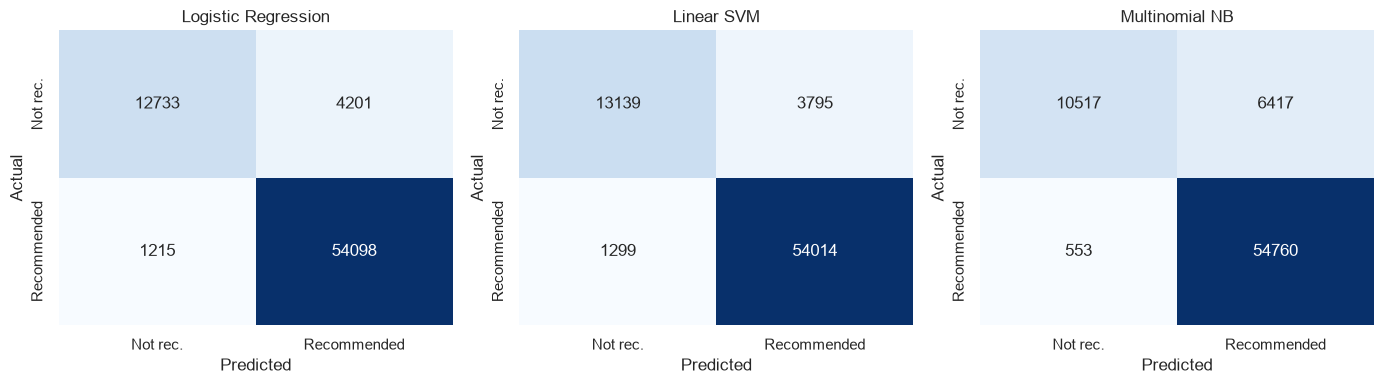
\includegraphics[width=\linewidth]{images/cb_classical_confmat.png}
\caption{Confusion matrices for the three classical models on the customer behaviour test
set.}
\end{figure}

\subsection{From-scratch deep learning model}

The network follows a $5000 \to 128 \to 32 \to 1$ architecture, with ReLU activations on
both hidden layers, a sigmoid output, and binary cross-entropy loss. The first hidden layer
is deliberately the widest relative to what follows it among the three applications in this
assignment, since the TF-IDF input is sparse and high-dimensional (5,000 columns, mostly
zero per row), and the first layer needs enough capacity to compress that information
usefully rather than bottlenecking it immediately. One practical detail is worth stating
explicitly: the input matrix is a scipy sparse matrix, and plain NumPy cannot operate on
sparse matrices directly, so training uses mini-batch gradient descent specifically so that
only one batch at a time needs to be densified, rather than converting the entire
288,986-row training matrix to a dense array in one shot (which would need several
gigabytes of memory just to hold it). Each epoch shuffles the training rows and steps
through them in batches of \texttt{BATCH\_SIZE = 1024}, one forward pass, one backward
pass, one gradient descent update per batch, so within a single epoch the weights update
many times rather than once. \texttt{EPOCHS = 25} and \texttt{LEARNING\_RATE = 0.1}
(higher than in the full-batch applications, since mini-batch updates happen far more
often per epoch) were chosen as a practical balance between letting the loss visibly
flatten out and keeping the runtime reasonable for a from-scratch NumPy loop over 291,000
training rows.

\begin{figure}[H]
\centering
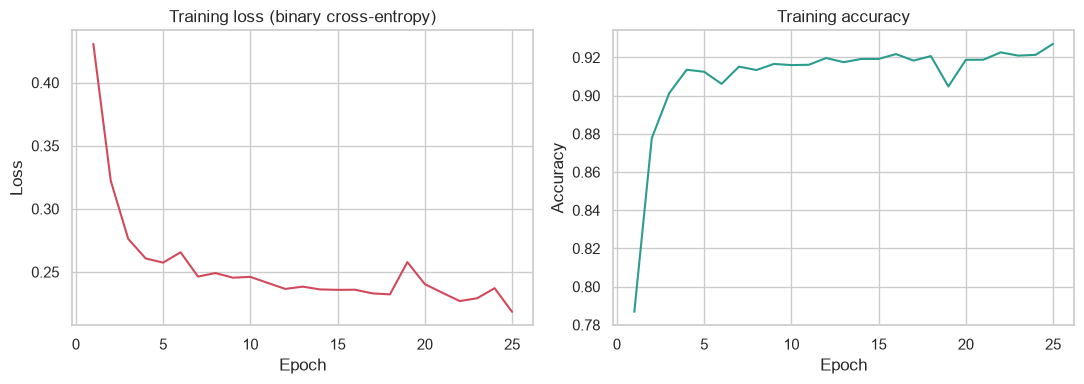
\includegraphics[width=\linewidth]{images/cb_dl_loss_acc.png}
\caption{Training loss (binary cross-entropy) and training accuracy per epoch for the
from-scratch customer behaviour network, evaluated on a fixed 20,000-row training subsample
each epoch to avoid a full extra forward pass purely for the curve.}
\end{figure}

\begin{table}[H]
\centering
\caption{Customer behaviour: from-scratch DL model results, test set}
\begin{tabular}{lrrrr}
\toprule
Model & Accuracy & Precision & Recall & F1 \\
\midrule
From-scratch DL & 0.9221 & 0.9238 & 0.9790 & 0.9506 \\
\bottomrule
\end{tabular}
\end{table}

\subsection{4-model comparison}

\begin{figure}[H]
\centering
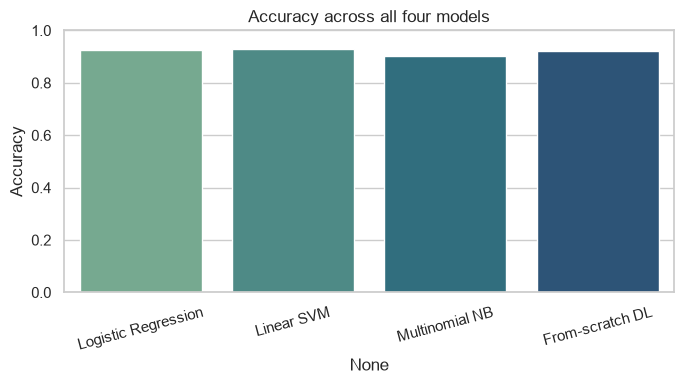
\includegraphics[width=0.7\linewidth]{images/cb_compare_accuracy.png}
\caption{Accuracy across all four customer behaviour models.}
\end{figure}

\begin{figure}[H]
\centering
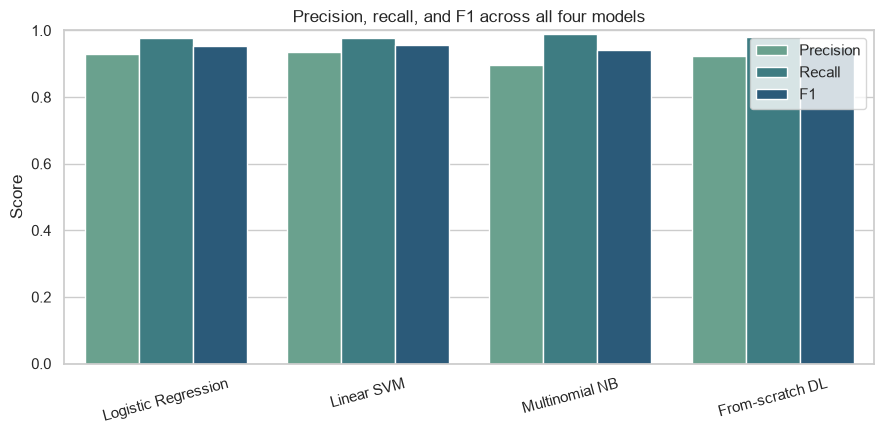
\includegraphics[width=\linewidth]{images/cb_compare_prf1.png}
\caption{Precision, recall, and F1 across all four customer behaviour models.}
\end{figure}

Linear SVM comes out slightly ahead by F1 at 0.9550, with Logistic Regression close behind
at 0.9523 and the from-scratch deep learning model right there alongside them at 0.9506.
Multinomial Naive Bayes trails at 0.9402, though ``trails'' is relative here, since every
model clears 94\% F1. Two separate effects explain why these scores sit this high, and both
were established in the EDA section above: the Review-to-Summary switch cut train/test
exact-text overlap from 99.1\% to 59.7\%, so these numbers are not mostly measuring
memorization of boilerplate strings, and roughly three in four rows carry a Summary whose
label stays highly consistent across every row sharing that exact text, a real property of
how sentiment language correlates with rating in this dataset rather than a flaw in the
evaluation.

Within that context, the three models built on a linear decision boundary over the TF-IDF
features, Logistic Regression, Linear SVM, and the from-scratch network's effectively-linear
first layer before any nonlinearity is applied, land within half a point of one another.
That closeness suggests the underlying task is close to linearly separable even on the
richer Summary text, once a review carries a handful of strongly positive or negative
words, and it is also why the deep learning model does not clearly outperform the linear
models: a nonlinear network's extra capacity only pays off when the true input-output
relationship is not already close to linear, and a bag-of-words sentiment signal mostly is.
Naive Bayes tells a different story: its recall is the highest of all four at 0.9900,
catching almost every genuinely recommended review, but its precision is the lowest at
0.8951, since without the ability to weigh combinations of words against each other the
way a linear model's coefficients can, it leans harder on individual strongly positive
words being present at all, and it never sees the \texttt{Price} feature either, a second,
smaller handicap. If anything is still holding the from-scratch network back from clearly
beating the linear models, it is the 5,000-term vocabulary cap needed to keep training
tractable, set against the classical models' access to the full, much larger vocabulary;
that the DL model still lands within half a point of Logistic Regression despite that
handicap is a reasonable sign the from-scratch implementation is learning a sound
representation.

\newpage
% ---------------------------------------------------------------------
\section{Cross-Application Comparison}
\label{sec:cross}
% ---------------------------------------------------------------------

Table \ref{tab:cross-app} summarizes all three applications by their primary metric
(Accuracy for the two classification tasks, $R^2$ for the regression task), across all four
models. Every cell simply transposes the per-application results tables from Sections
\ref{sec:diabetes}, \ref{sec:house_price}, and \ref{sec:customer_behaviour}, rather than
introducing new analysis.

\begin{table}[H]
\centering
\caption{Cross-application summary: primary metric, all 3 datasets x 4 models}
\label{tab:cross-app}
\begin{tabular}{llrr}
\toprule
Application & Metric & Model & Score \\
\midrule
\multirow{4}{*}{Diabetes}
  & \multirow{4}{*}{Accuracy} & Logistic Regression & 0.7236 \\
  & & Random Forest & 0.7146 \\
  & & Gradient Boosting & 0.7149 \\
  & & From-scratch DL & \textbf{0.7343} \\
\midrule
\multirow{4}{*}{House price}
  & \multirow{4}{*}{$R^2$} & Linear Regression & $-48.3632$ \\
  & & Random Forest & \textbf{0.3980} \\
  & & Gradient Boosting & 0.2397 \\
  & & From-scratch DL & $-1.1044$ \\
\midrule
\multirow{4}{*}{Customer behaviour}
  & \multirow{4}{*}{Accuracy} & Logistic Regression & 0.9250 \\
  & & Linear SVM & \textbf{0.9295} \\
  & & Multinomial NB & 0.9035 \\
  & & From-scratch DL & 0.9221 \\
\bottomrule
\end{tabular}
\end{table}

\noindent\textit{Each application's three classical models differ, per the model choices
justified in its own section above (Random Forest and Gradient Boosting for the two
tabular tasks; Linear SVM and Multinomial Naive Bayes in place of tree models for the
sparse TF-IDF text task), so this table lists each application's actual models rather
than forcing them into shared generic column headers. Bold marks the winning score in
each application.}

The from-scratch deep learning model wins outright on one of the three applications
(diabetes) and lands within roughly half a percentage point of the best classical model on
a second (customer behaviour), while trailing clearly on the third (house price). This
pattern, and the reasons behind it, is taken up in the discussion below.

% ---------------------------------------------------------------------
\section{Discussion: What Changed from Assignment 02}
\label{sec:discussion}
% ---------------------------------------------------------------------

\subsection{The same three problems, a new model added}

Every application preserved the same problem framing as Assignment 02: diabetes binary
classification, house price regression, and review recommend/not classification, each run
on a new dataset (a second BRFSS survey year for diabetes, a larger US-market sample for
house price, a different e-commerce platform for customer behaviour). The genuinely new
ingredient this round is the from-scratch deep learning model, evaluated against the same
three classical models used before, but now as one of four models per application instead
of the only comparison point.

\subsection{What got harder: training time with no framework to lean on}

Training a dense feedforward network with a pure-NumPy loop, over hundreds of thousands of
rows, with no GPU and no vectorized-framework tricks beyond what NumPy itself provides, is
noticeably slower and more fragile than simply calling \code{model.fit()} on a scikit-learn
estimator. The diabetes and house price networks used full-batch gradient descent (the
entire training matrix fits comfortably in memory as a dense array), while the customer
behaviour network had to switch to mini-batch gradient descent specifically because its
5,000-column TF-IDF input, if densified all at once across 288,986 rows, would need several
gigabytes of memory just to hold. Finding a stable learning rate for each application also
took real, direct benchmarking rather than a single default choice: the house price network
suffered a dead-ReLU collapse at a learning rate of 0.3 before 0.01 was found to train
stably, and the diabetes rate was chosen by comparing candidate rates directly rather than
guessing.

\subsection{Did the from-scratch model actually beat the classical models?}

The honest answer varies by application, and that variation is itself the useful finding.
On diabetes, the from-scratch network won outright by F1 (0.4648, narrowly ahead of all
three classical models once balanced weighting was applied to every model). On customer
behaviour, it landed within half a point of the best classical model (0.9506 vs. Linear
SVM's 0.9550) despite reading only 5,000 of the full 416,770-term vocabulary available to
the classical models, a deliberately accepted trade-off to keep a dense NumPy forward and
backward pass tractable rather than a modeling failure. On house price, it placed third,
ahead of Linear Regression but well behind both tree ensembles ($R^2 = -1.1044$ against
Random Forest's 0.3980), because its output layer shares Linear Regression's unbounded
linear structure, with no ceiling the way a tree's leaf-average prediction has, on a target
whose raw-dollar space is extremely heavy-tailed. Neither the customer behaviour vocabulary
cap nor the house price extrapolation weakness is a bug; both are known, explainable
limitations, a small network against tree ensembles on a heavy-tailed regression target,
and a deliberately narrower vocabulary against a full-vocabulary linear model, worth naming
plainly rather than glossing over.

\subsection{What building the optimizer by hand exposed}

One finding deserves particular attention because it is specifically invisible when calling
\code{model.fit()} on a packaged implementation: plain gradient descent
(\texttt{W -= lr * dW}, no per-parameter adaptive scaling, no Adam, nothing a framework
quietly handles) offers no defense against a feature sitting on a wildly different numeric
scale than the rest of the input. This surfaced independently while building two of the
three from-scratch networks in this assignment.

In diabetes, the \verb|year| column was initially left as the literal 2019/2020 integer
rather than mapped to a 0/1 flag. Left that way, it entered the feature matrix at a scale of
roughly 2020, dwarfing every standardized or small-integer feature beside it, and blew up
the forward pass: the sigmoid overflowed at epoch 1, with a recorded loss of 17.49. Mapping
\verb|year| to a binary flag (2020 vs. 2019) fixed this completely, and is also the correct
encoding on its own merits for a field with only two possible values, where a second one-hot
column would just be a redundant mirror of the first.

In house price, \verb|city_freq| (a raw count running into the thousands for popular
cities) would have entered the feature matrix unscaled, next to one-hot flags and
already-standardized fields, the same class of problem. This one was caught by inspection
before the network was ever executed, and fixed by folding \verb|city_freq| into the same
\verb|StandardScaler| step as the other continuous columns, after first applying
\verb|log1p| to tame its own heavy tail (the same fix independently needed for
\verb|acre_lot| and \verb|house_size|, both heavy-tailed counts whose raw scale produced
double-digit standardized z-scores).

In both cases, every classical model trained on the exact same feature matrix remained
entirely unaffected: scikit-learn's solvers and the tree ensembles are either scale-
invariant (trees split on raw thresholds regardless of scale) or considerably more robust
to ill-conditioning than a hand-written gradient descent loop with a fixed step size. This
is precisely the kind of failure mode a packaged implementation absorbs silently, sensible
default preprocessing, adaptive optimizers, or internal gradient clipping, none of which
existed here to catch it, so it was only discoverable by building the optimizer by hand.

% ---------------------------------------------------------------------
\section{Conclusion}
% ---------------------------------------------------------------------

This assignment extended three intelligent systems, diabetes risk screening, house price
prediction, and e-commerce review classification, each run on a genuinely larger dataset
than Assignment 02, with a fourth model added per application: a feedforward neural network
whose forward propagation, loss, backpropagation, and gradient descent update were all
derived by hand in NumPy, with no autograd and no deep learning framework involved. The
from-scratch implementation proved competitive rather than merely functional, winning
outright on the diabetes task and landing within half a point of the best classical model
on customer behaviour, while a clear, well-understood limitation, an unbounded linear
output on a heavy-tailed regression target, accounts for its weaker showing on house price.
Deriving every gradient by hand, rather than calling a packaged \code{model.fit()}, made it
possible to state precisely why the network wins, ties, or loses on each task, and also
surfaced a failure mode a packaged implementation would have silently absorbed: a single
unscaled feature is enough to derail full-batch gradient descent even when every classical
model trained on the identical feature matrix remains unaffected. The same
representation-learning and optimization framework from Section \ref{sec:lecture} explains
every one of these outcomes once the architecture, activation choice, and loss for each
application are made explicit rather than left buried inside a library.

% ---------------------------------------------------------------------
\section{Reproducibility}
% ---------------------------------------------------------------------

\subsection{Environment}

\begingroup\sloppy\emergencystretch=3em
All three notebooks were built and executed in a dedicated virtual environment at
\texttt{assignment\_03/.venv} (Python, registered as Jupyter kernel
\texttt{assignment\_03}), with the following key package versions: numpy 2.5.3, pandas
3.0.5, scikit-learn 1.9.1, scipy 1.18.1, matplotlib 3.11.2, seaborn 0.13.2, jupyter,
nbconvert 7.16.6. No \code{tensorflow}, \code{torch}, or \code{keras} package is
imported anywhere in the three notebooks. \texttt{RANDOM\_SEED = 42} is fixed in every
notebook for every split, shuffle, and weight initialization.
\par\endgroup

\subsection{Re-running a notebook end to end}

Each application's notebook is self-contained and can be re-run end to end from its own
directory using:
\begin{footnotesize}
\begin{verbatim}
../.venv/Scripts/python.exe -m jupyter nbconvert \
    --to notebook --execute --inplace \
    notebook/<app>.ipynb --ExecutePreprocessor.timeout=1800
\end{verbatim}
\end{footnotesize}
replacing \texttt{<app>} with \texttt{diabetes}, \texttt{house\_price}, or
\texttt{customer\_behaviour}. Each notebook ends by saving its trained artifacts to its
own \texttt{model/} directory:
\begin{itemize}[nosep]
  \item \texttt{model\_pipeline.joblib}: the best classical model, plus its fitted
    scaler/vectorizer.
  \item \texttt{feature\_names.joblib}: the post-encoding feature column order.
  \item \texttt{input\_schema.json}: documented input fields and target.
  \item \texttt{dl\_weights.npz}: the from-scratch network's trained weights and biases.
\end{itemize}
followed by a reload-and-verify cell that reloads both artifacts and checks that their
predictions match the in-memory versions computed during that same run. No API, web, or
mobile layer is included in this assignment, so no run commands beyond notebook execution
are required.

\end{document}
